This chapter will present the actual implementation of our model in the \textit{Simulink} environment together with its open loop analysis of stability.

\section{Implementation}
\subsection{Motors}
The model of the motors is displayed in Figure \ref{motorr}. Each transfer function was obtaineed by putting the coefficients obtained in Section x in place. The deadzone for each motor was also added to the simulation. The output of the system is represented by the angular velocities of the propellers. 

\begin{figure}[H]
  \centering
    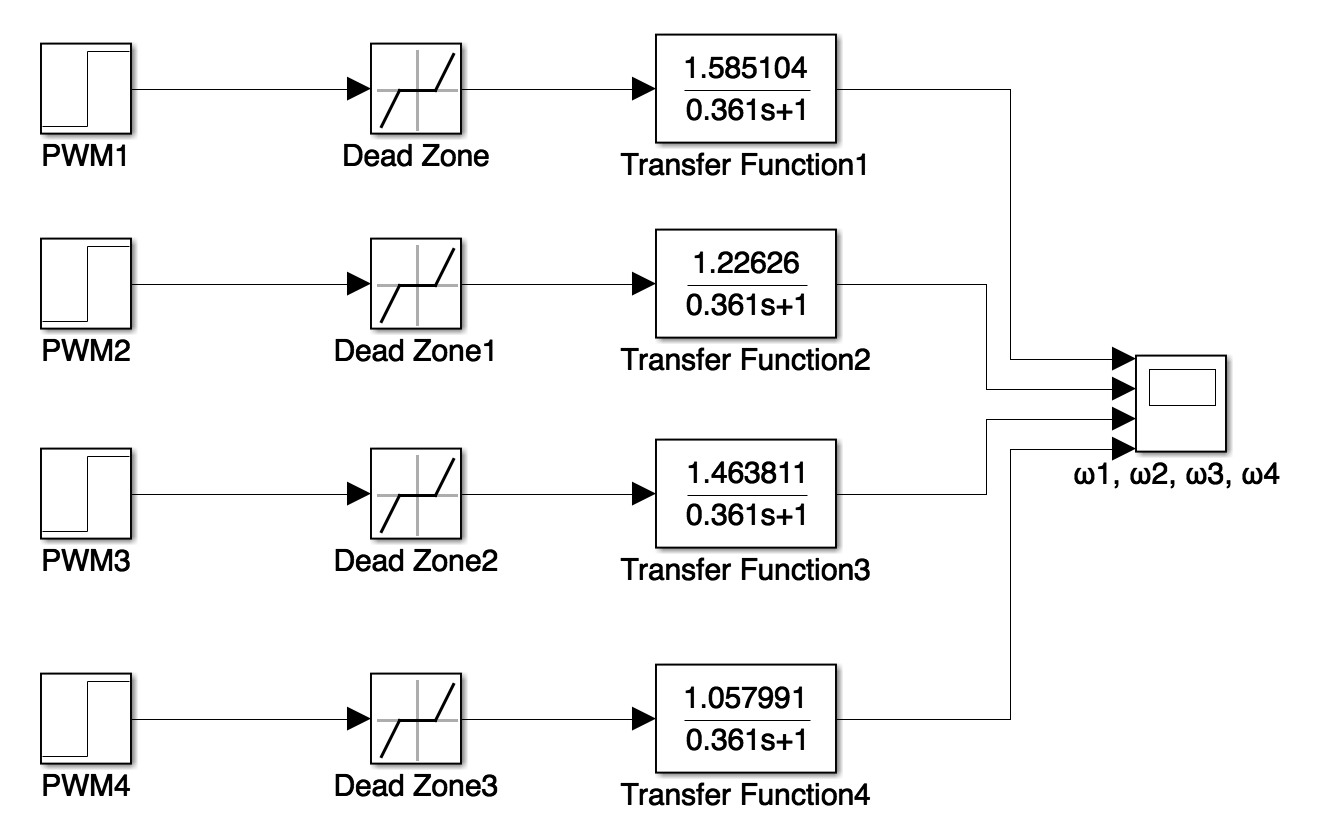
\includegraphics[width=1.0\textwidth]{images/simulinkmotor.png}
	\caption{Implementation of the motors' model.}
	\label{motorr}
\end{figure}

By giving the PWM values from Table \ref{motorCoeffs}, the simulation shows angular velocity of all four motors. It can be seen in Figure \ref{motorScope} that the speeds still do not match perfectly. This is because none of the functions are linear, giving only the approximations of the coefficients used in the model and not exact values. As such, some controller will need to be implemented to try and compensate for the differences.

\begin{figure}[H]
  \centering
    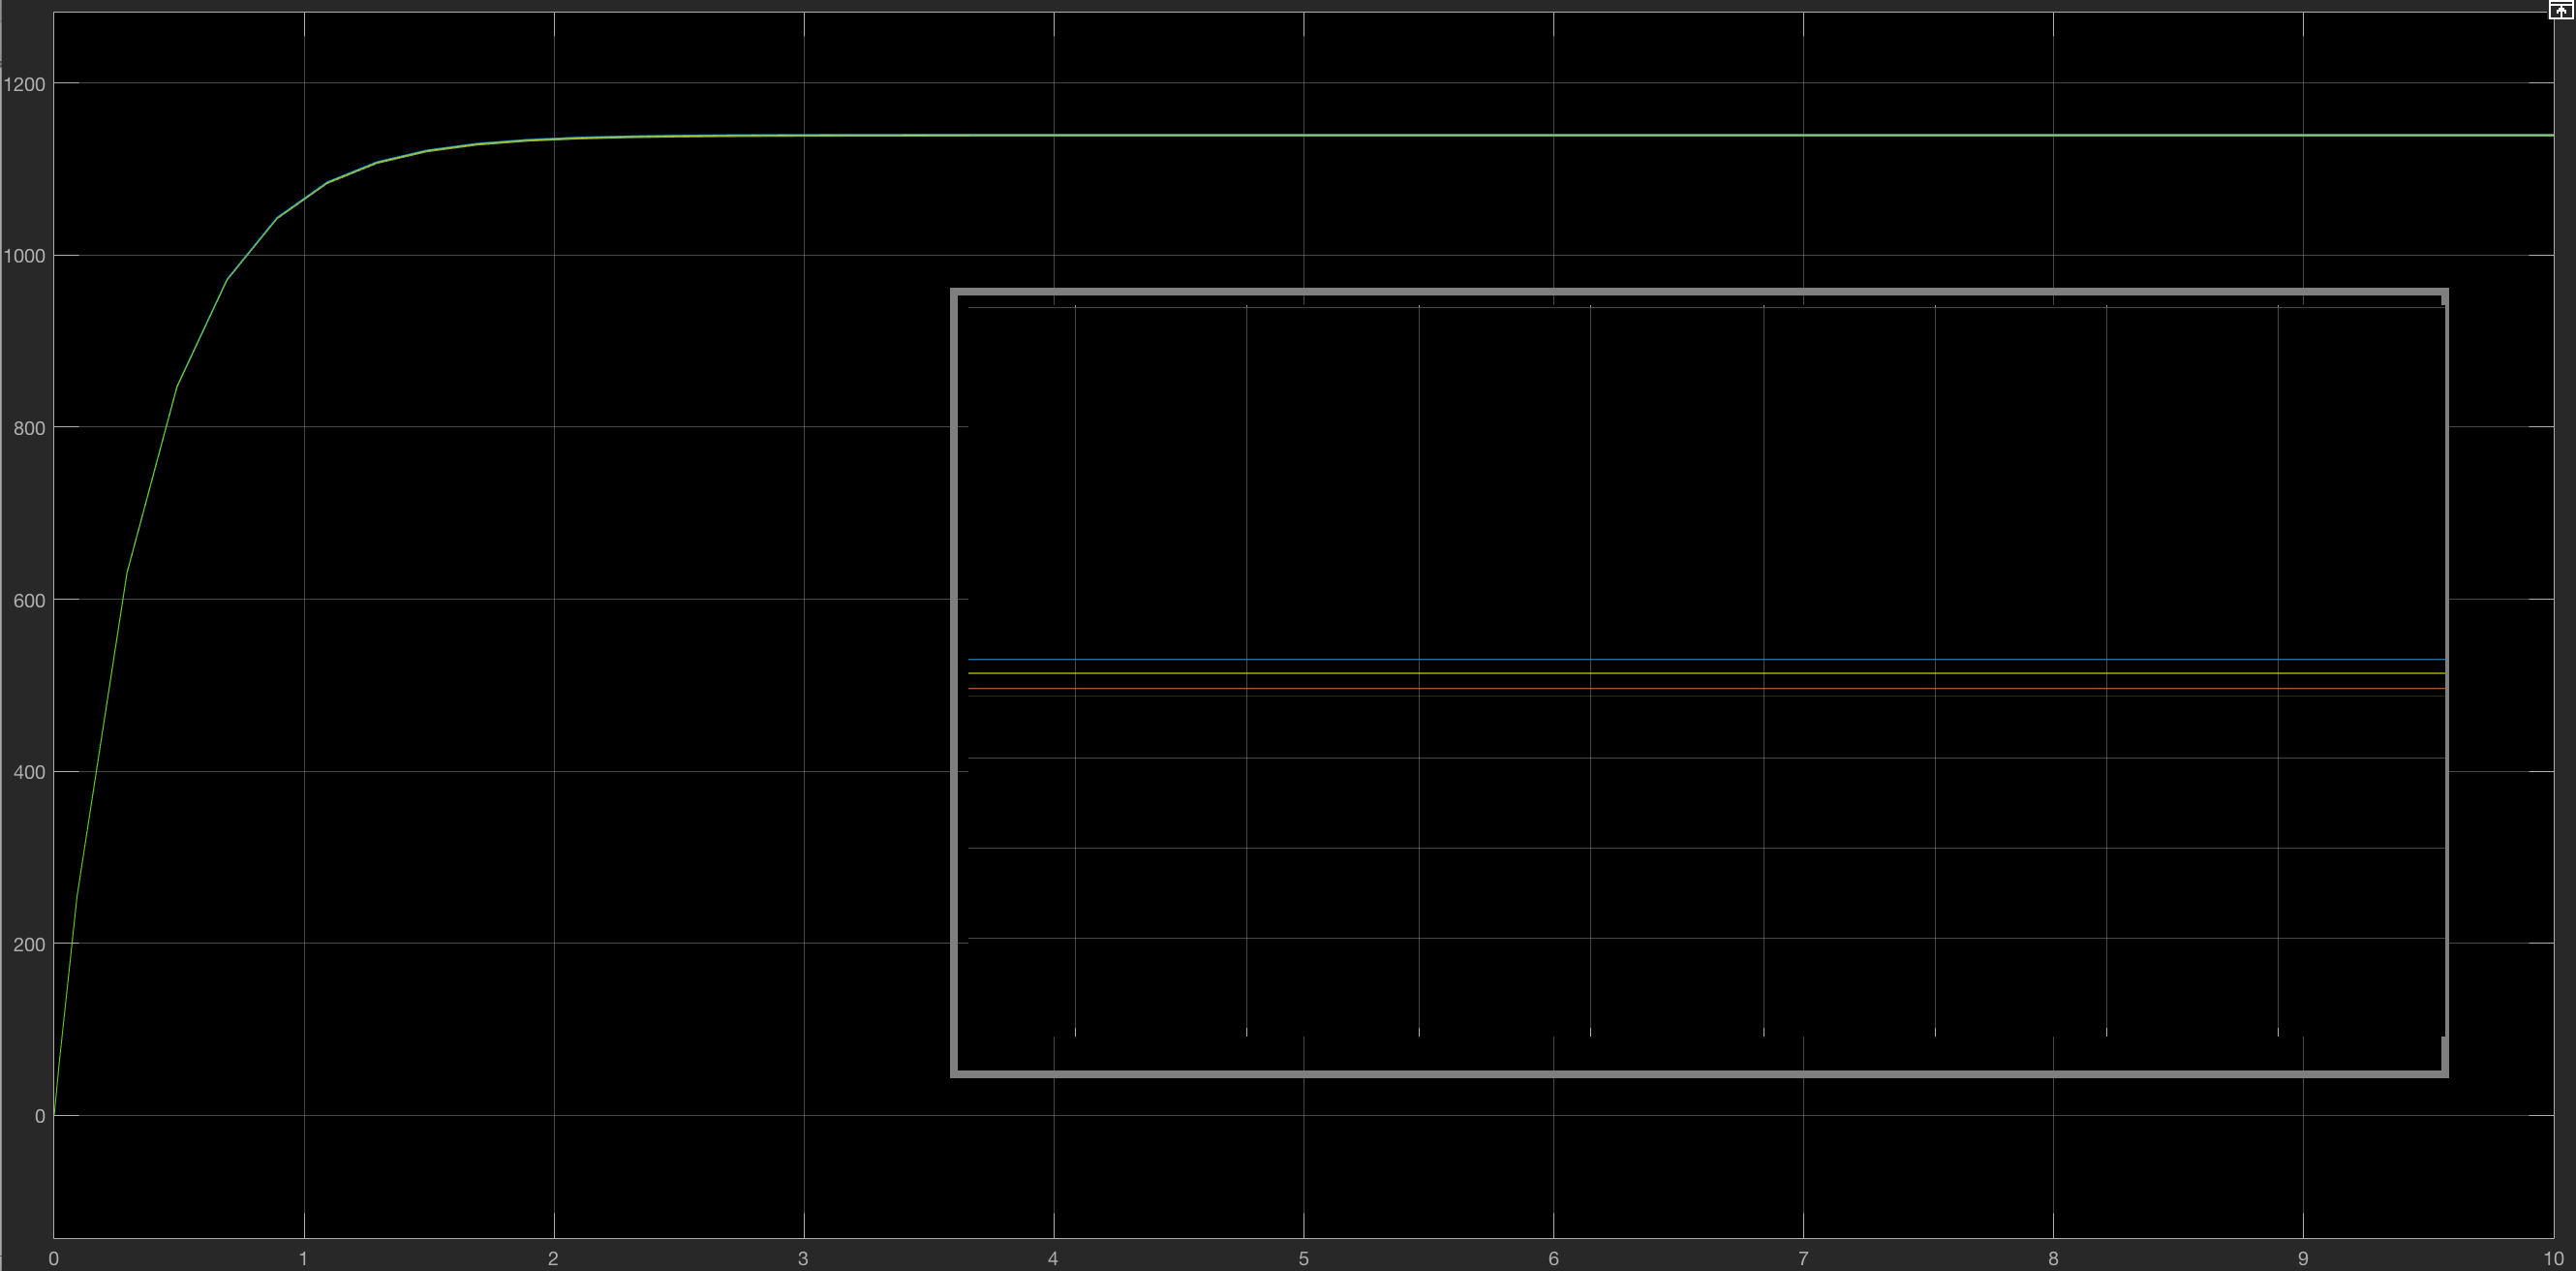
\includegraphics[width=1\textwidth]{images/scopewithcloseup.png}
	\caption{The Output of the Model and a Close Up.}
	\label{motorScope}
\end{figure}

\subsection{Model Simulation}

\begin{figure}[H]
  \centering
    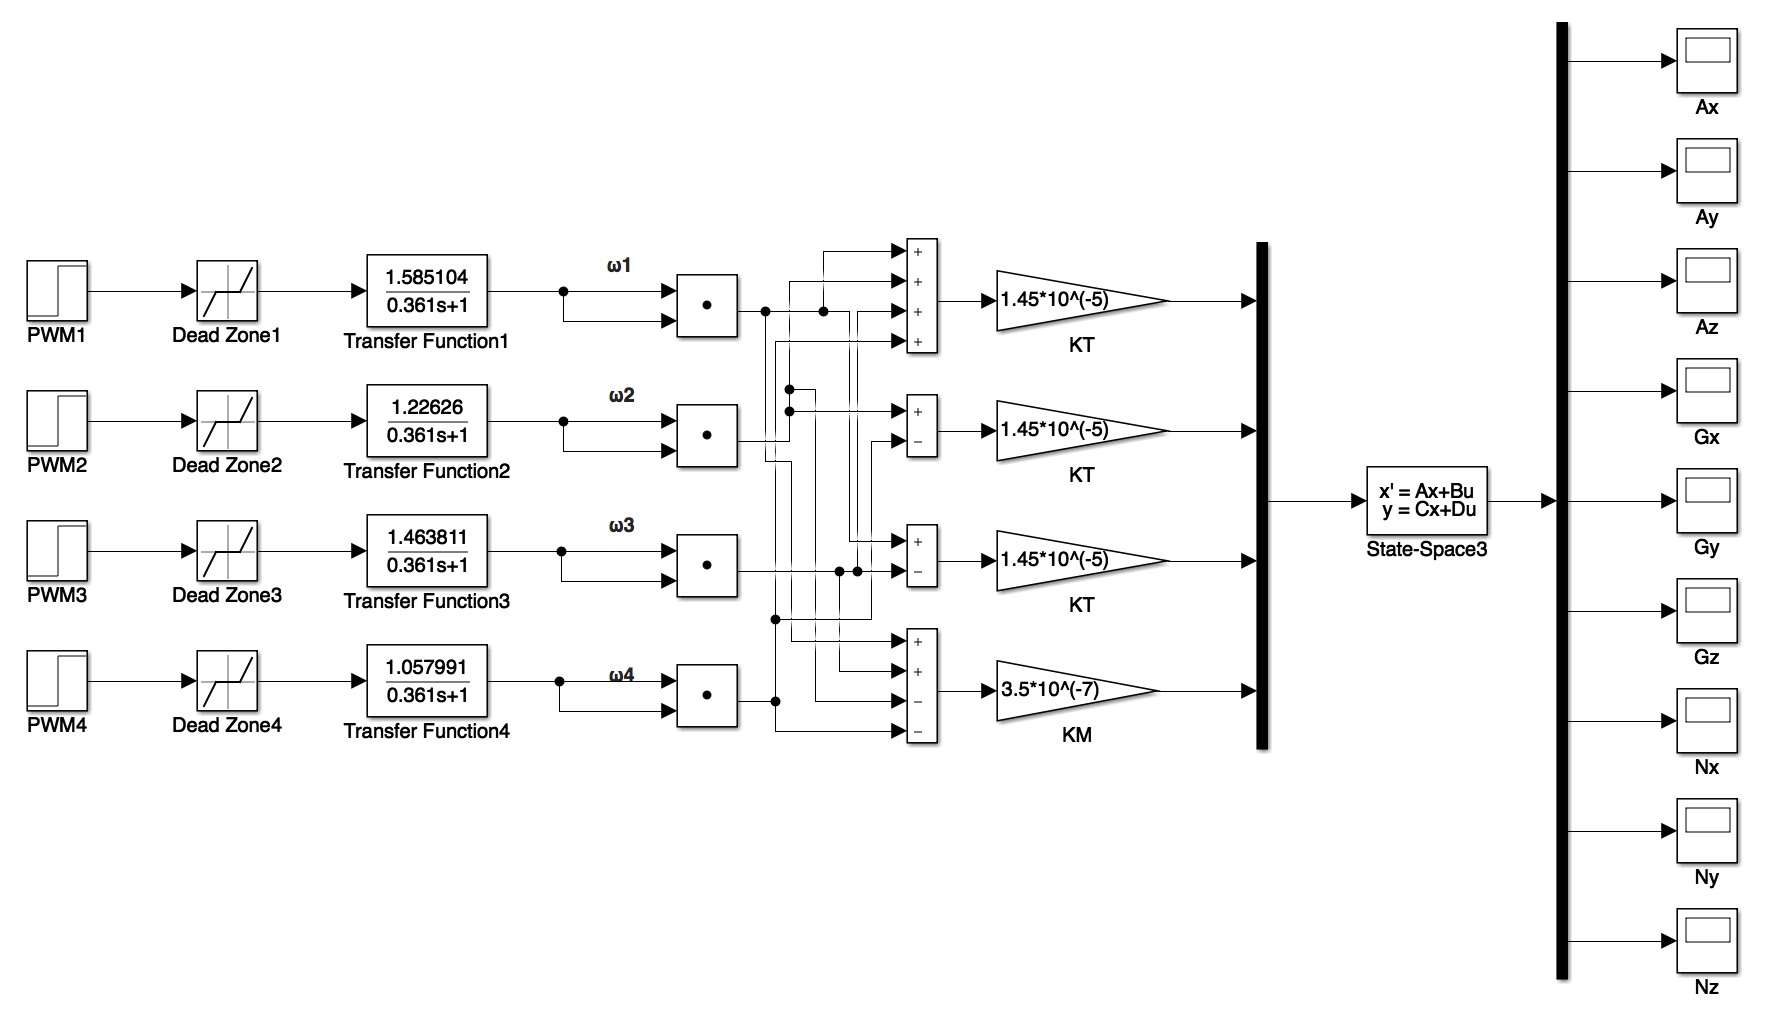
\includegraphics[width=1\textwidth]{images/openloop.png}
	\caption{Implementation of the full model.}
	\label{openloop}
\end{figure}

Open loop response:

Ax,Ay,Az,Nx,Nz:

\begin{figure}[H]
  \centering
    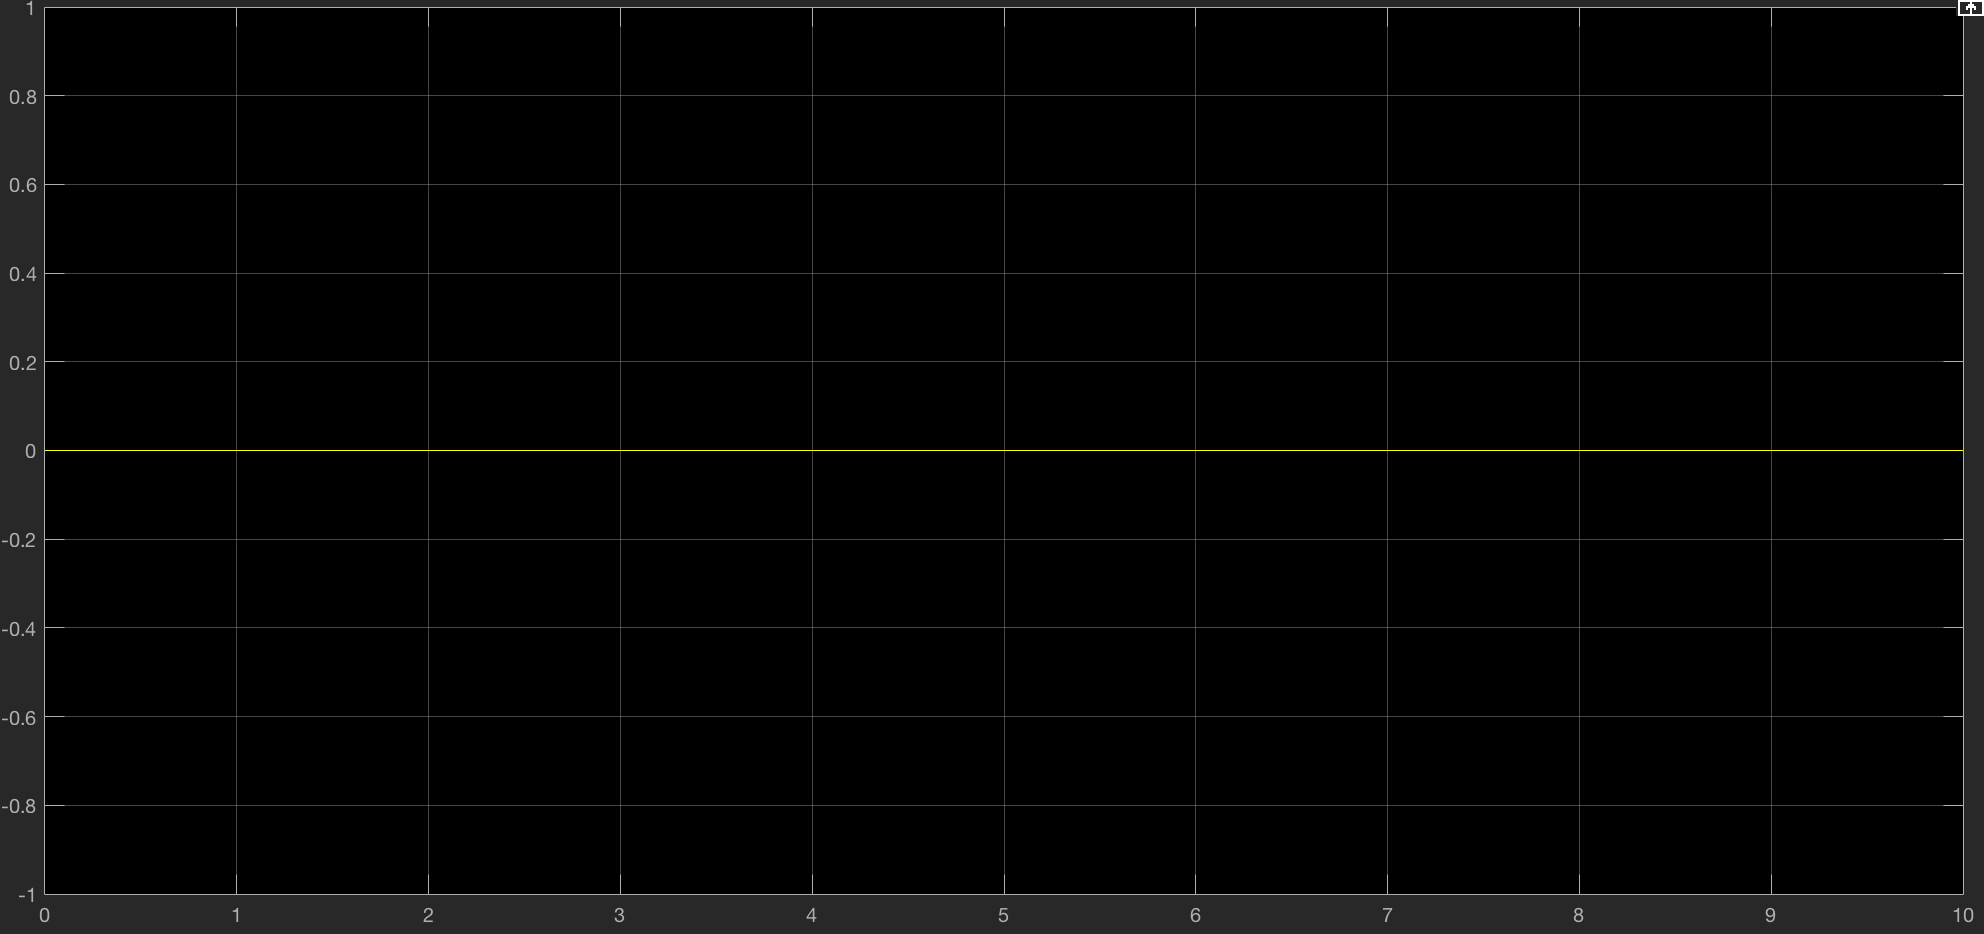
\includegraphics[width=1\textwidth]{images/Ax.png}
	\caption{something.}
	\label{openloop1}
\end{figure}

\begin{figure}[H]
  \centering
    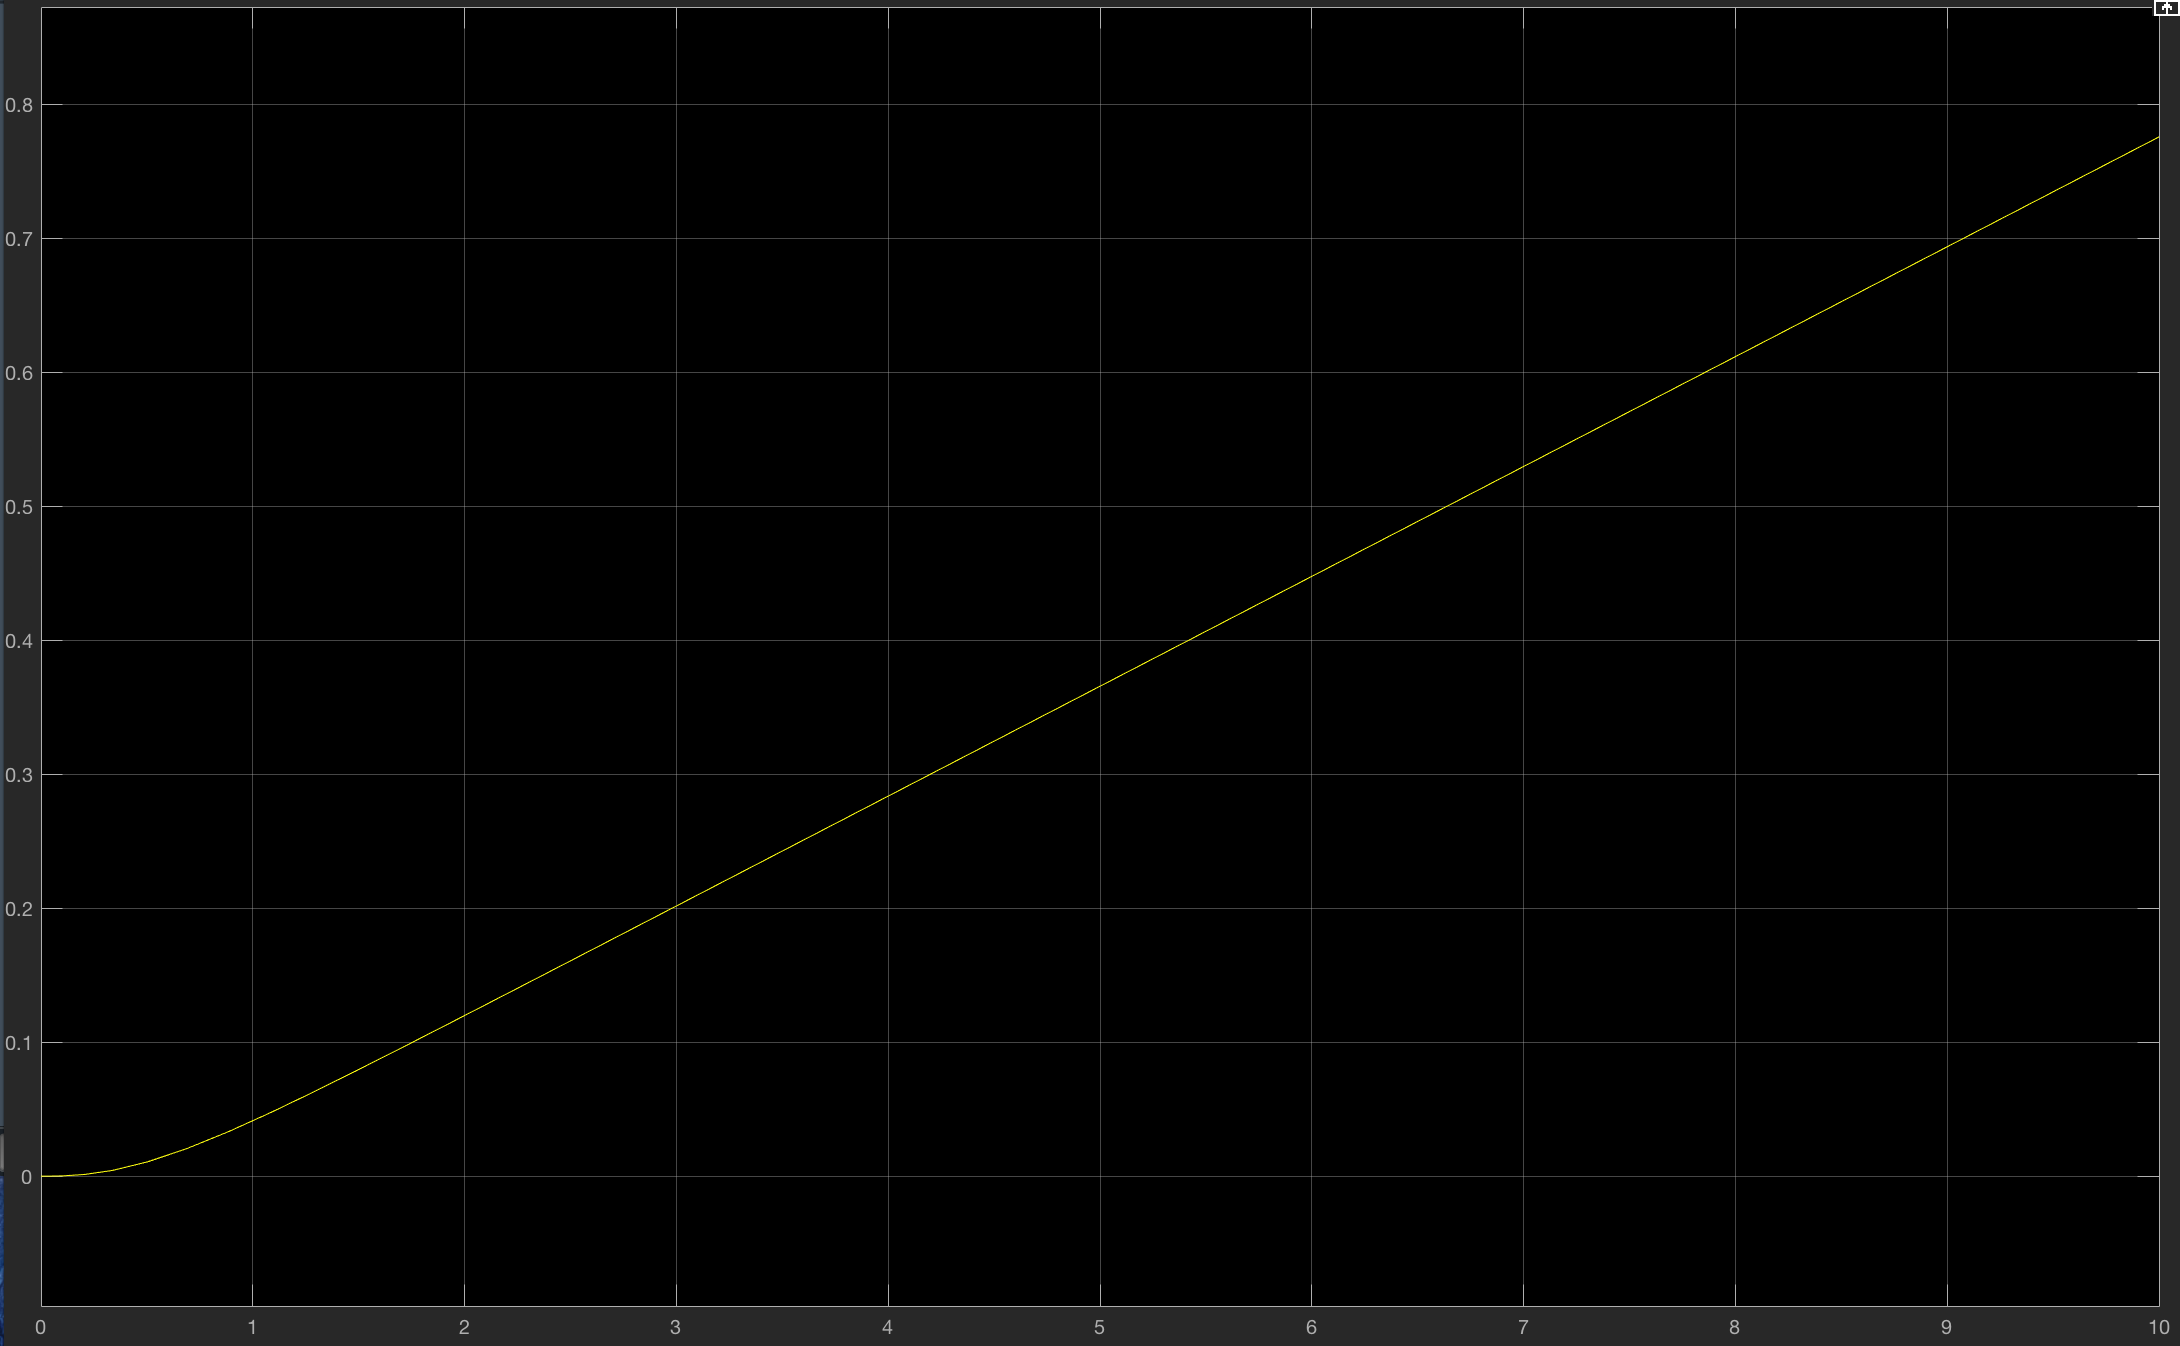
\includegraphics[width=1\textwidth]{images/Gx.png}
	\caption{Implementation of the full model.}
	\label{openloop2}
\end{figure}

\begin{figure}[H]
  \centering
    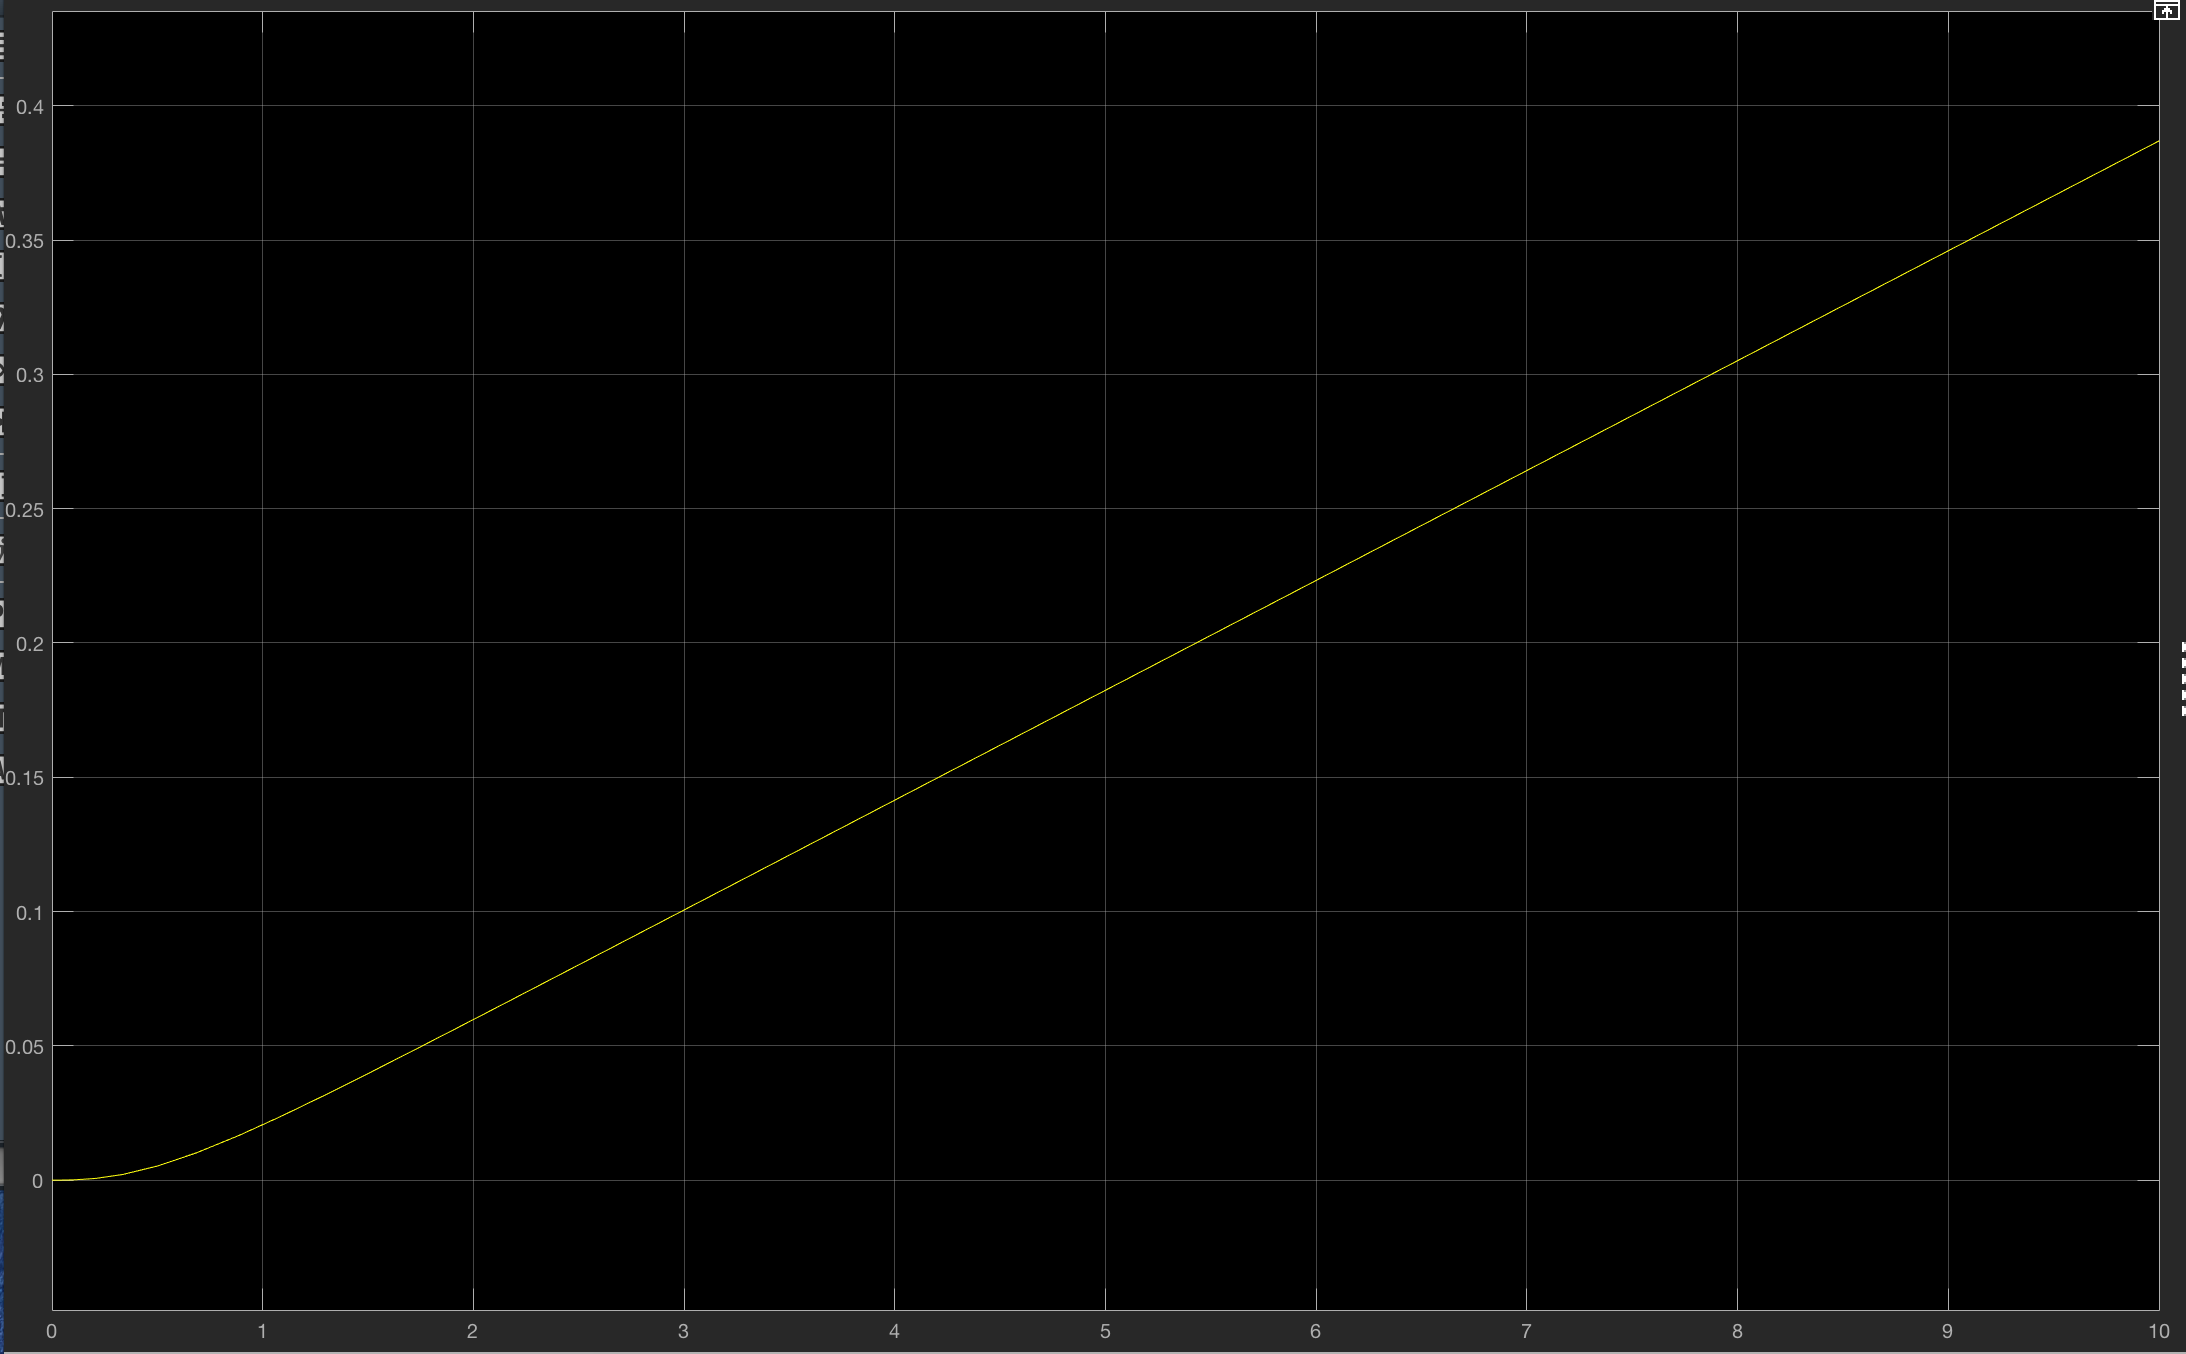
\includegraphics[width=1\textwidth]{images/Gy.png}
	\caption{Implementation of the full model.}
	\label{openloop3}
\end{figure}

\begin{figure}[H]
  \centering
    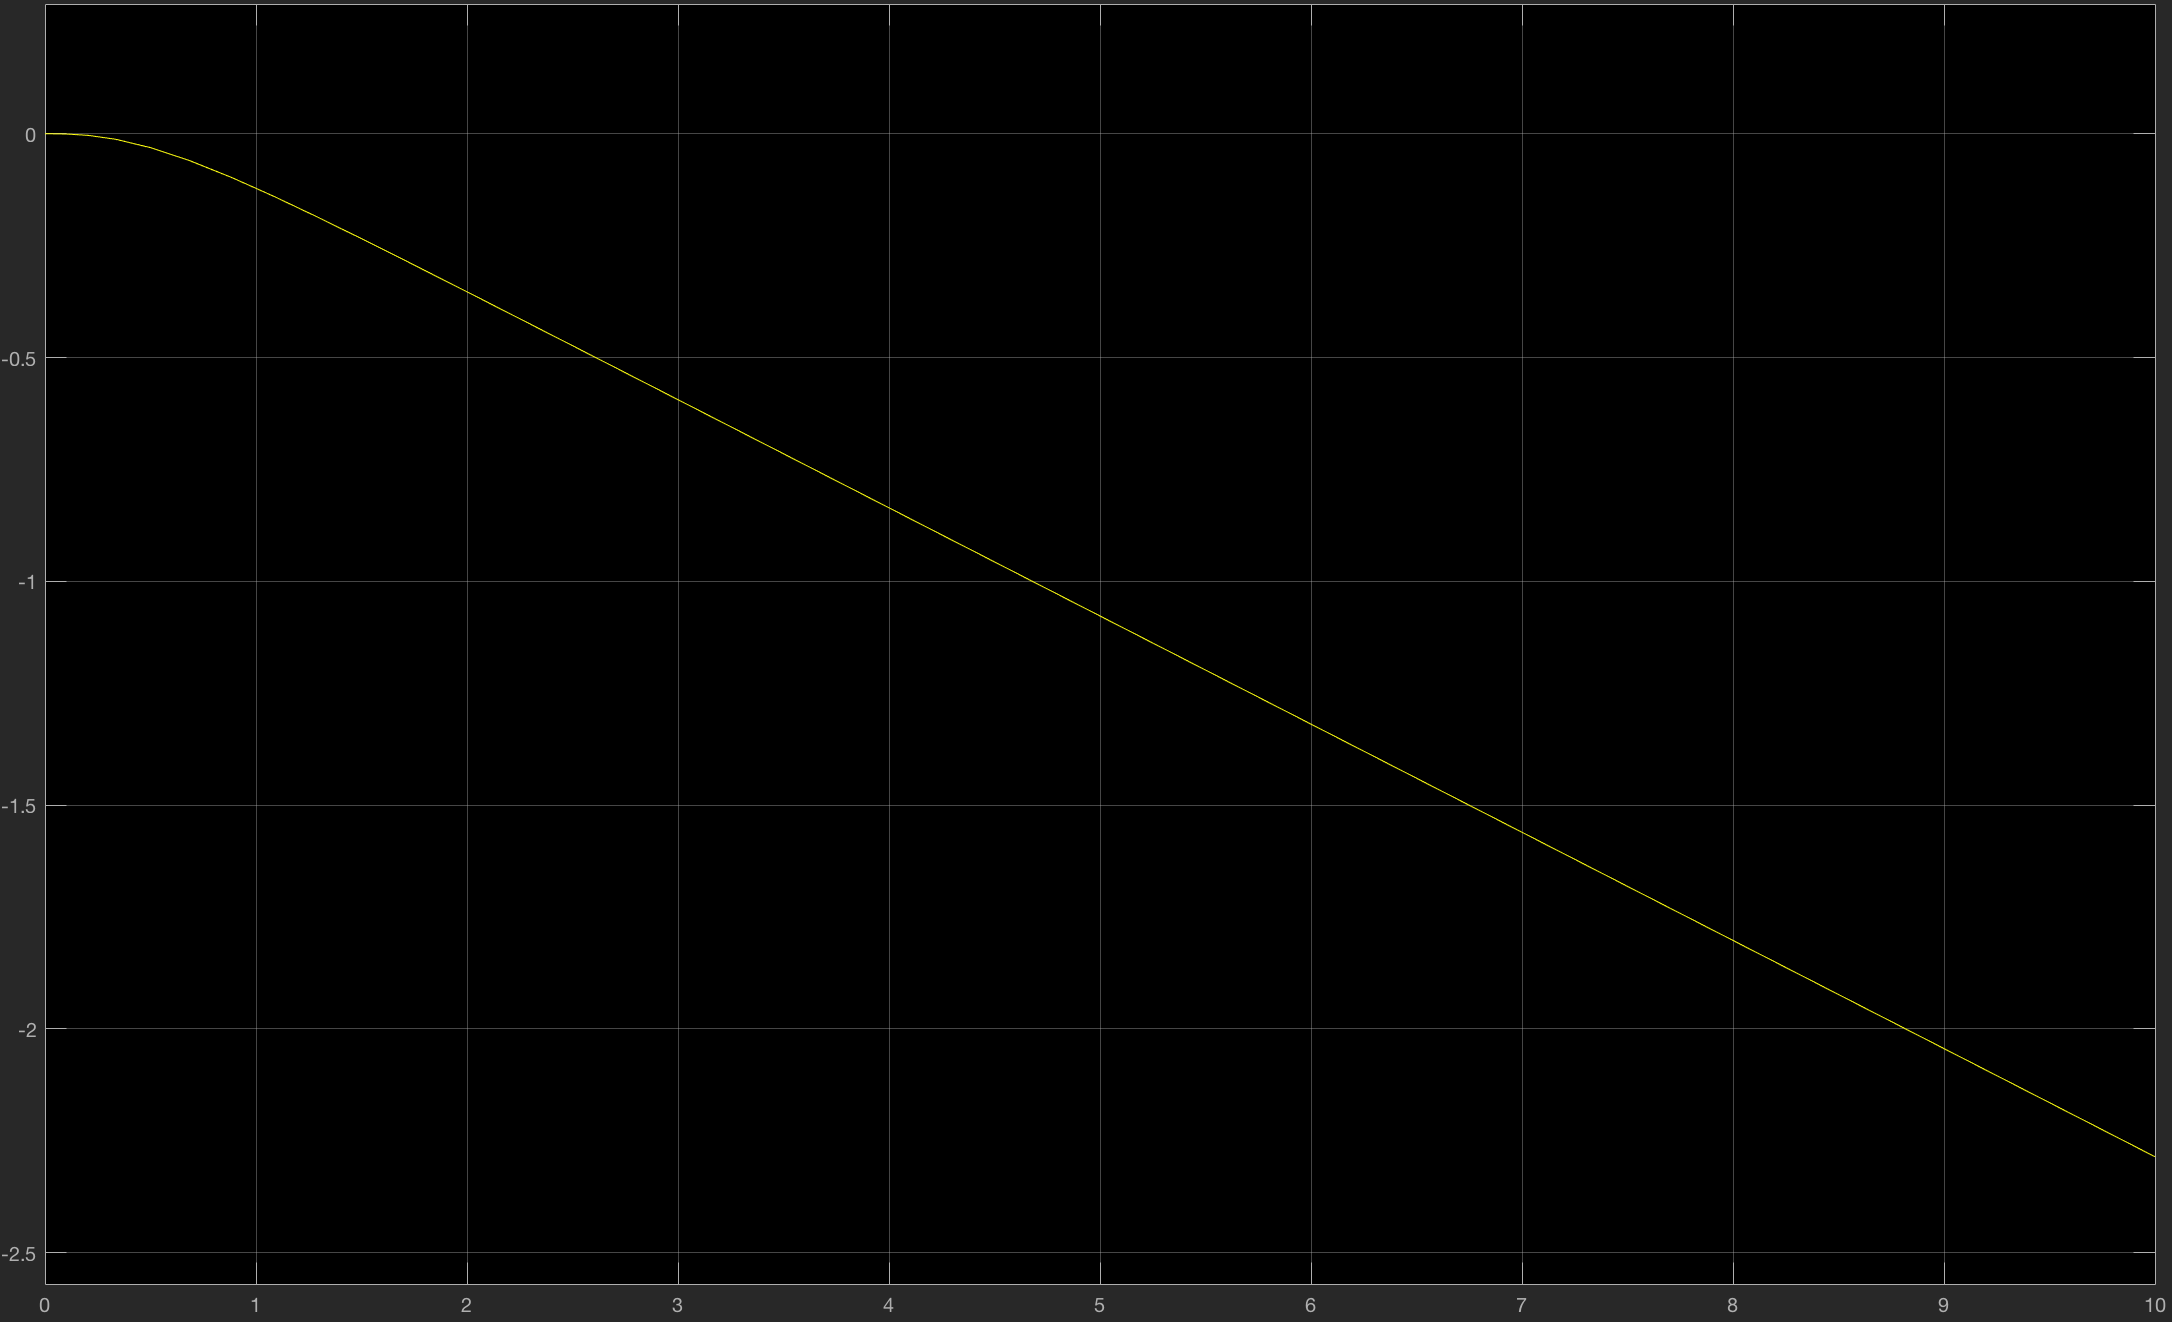
\includegraphics[width=1\textwidth]{images/Gz.png}
	\caption{Implementation of the full model.}
	\label{openloop4}
\end{figure}

\begin{figure}[H]
  \centering
    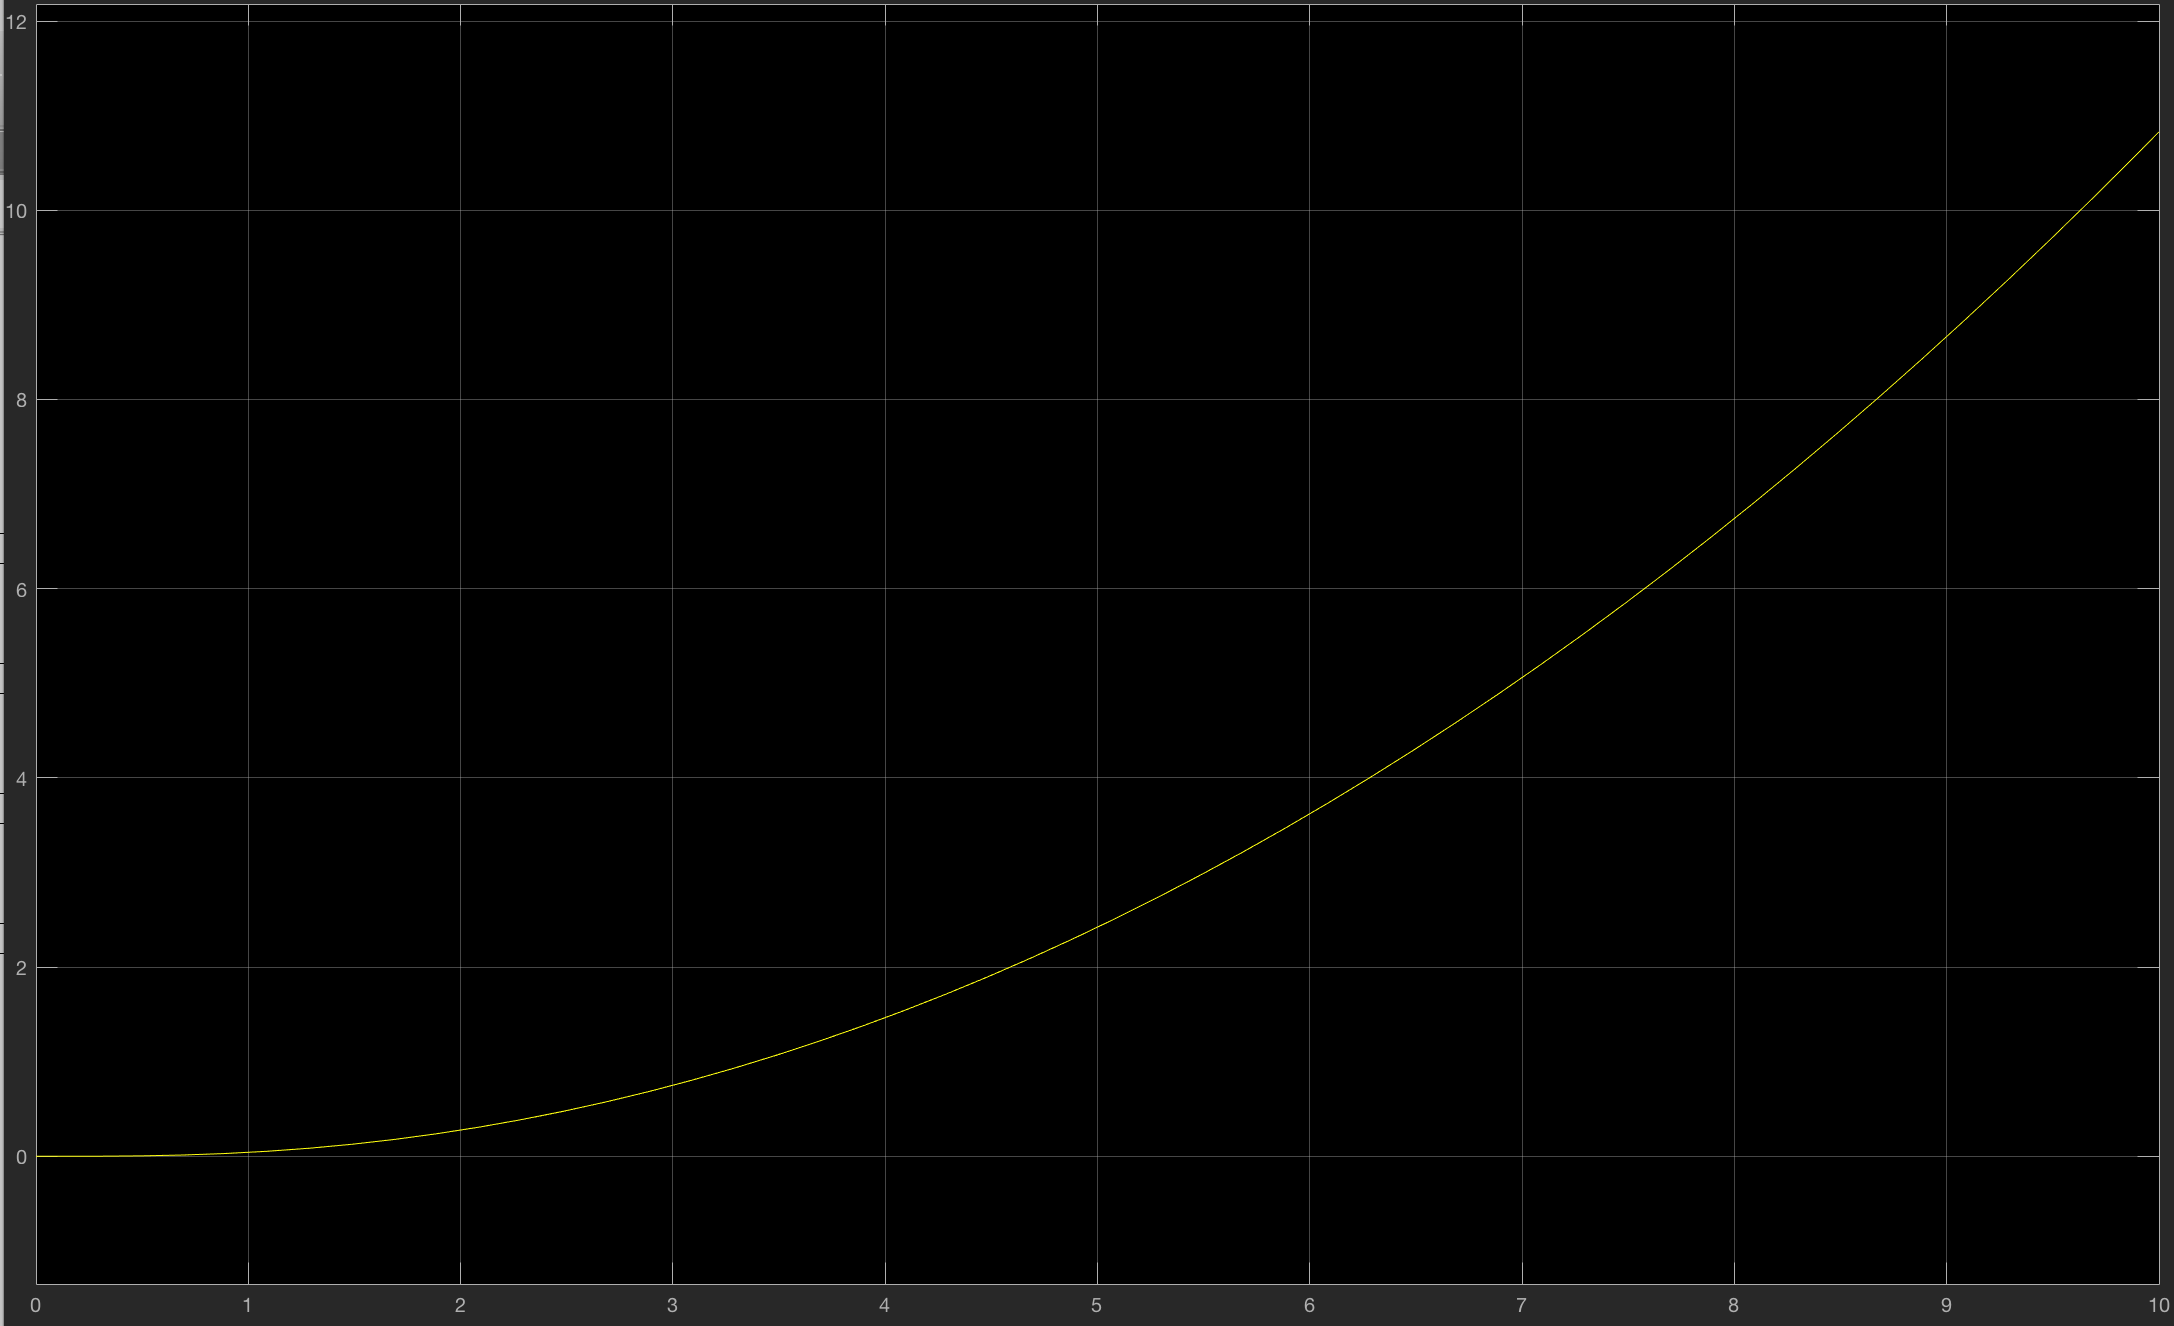
\includegraphics[width=1\textwidth]{images/Ny.png}
	\caption{Implementation of the full model.}
	\label{openloop5}
\end{figure}

